\documentclass[12pt]{article}

\usepackage[margin=0.5in]{geometry} 
\usepackage{amsmath,amsthm,amssymb,color}
\usepackage{graphicx}
\usepackage{mathtools}
\usepackage[section]{placeins}
\usepackage{listings}
\usepackage{mathdots}
\usepackage{centernot}
\usepackage{algorithm}
\usepackage[noend]{algpseudocode}
\usepackage{csquotes}
\usepackage[table,xcdraw]{xcolor}
\usepackage{enumerate}
\usepackage{tikz}
\usetikzlibrary{calc}
\usepackage{bbm}
\usetikzlibrary{arrows, shapes}
\usetikzlibrary{patterns}
\usepackage{relsize}

\usetikzlibrary{decorations.pathreplacing}
\allowdisplaybreaks


\usepackage{hyperref}
\hypersetup{
    colorlinks,
    citecolor=black,
    filecolor=black,
    linkcolor=black,
    urlcolor=black
}

\DeclarePairedDelimiter\ceil{\lceil}{\rceil}
\DeclarePairedDelimiter\floor{\lfloor}{\rfloor}
 
\newcommand\scalemath[2]{\scalebox{#1}{\mbox{\ensuremath{\displaystyle #2}}}}



\begin{document}

\begin{figure}

\begin{center}
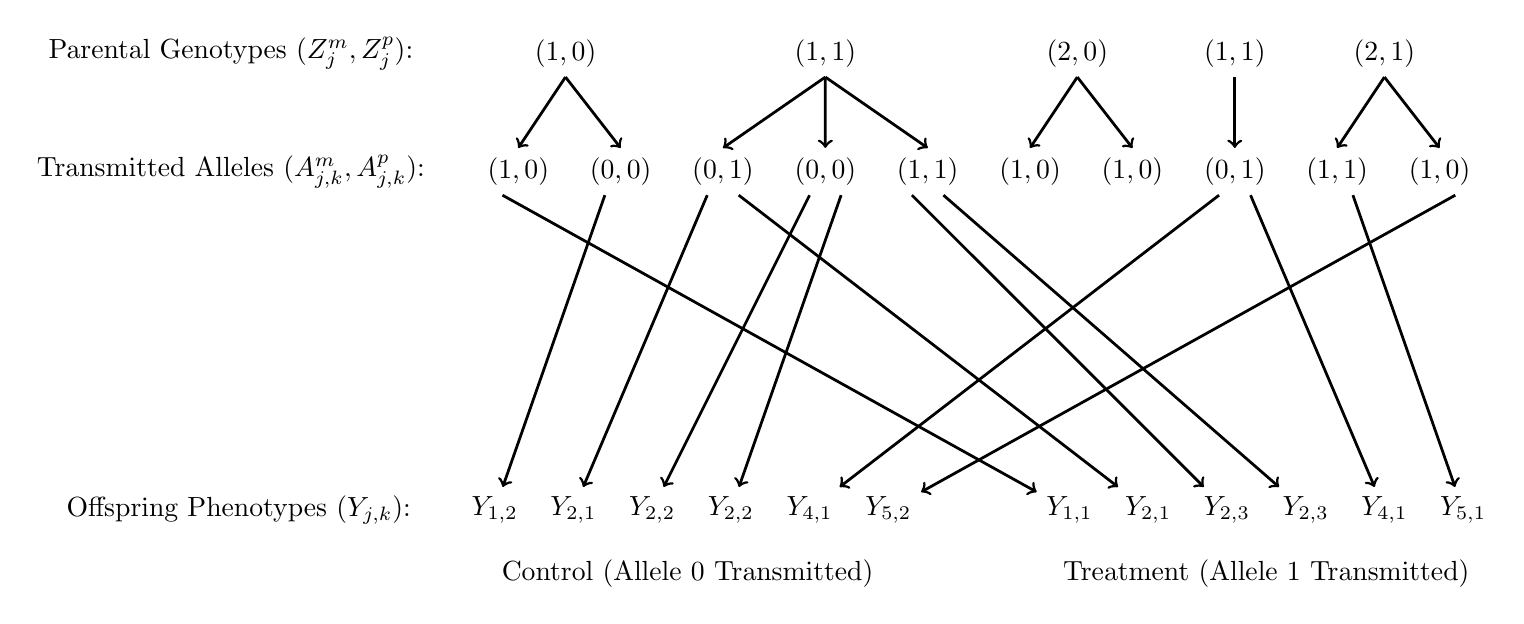
\begin{tikzpicture}[scale = 1]

\tikzstyle{vertex_P}=[rectangle,fill=blue, opacity = 0.5, text width = 6mm, text height = 6mm]
\tikzstyle{vertex_M}=[diamond,fill=red, opacity = 0.5, text width = 7mm]
\tikzstyle{vertex_t}=[circle,fill=black, opacity = 1, text width = 3mm]
\tikzstyle{vertex_c}=[circle,fill=black, opacity = 1, text width = 3mm]

\coordinate (y1) at (-6.5, 3);
\coordinate (y2) at (-5.2, 3);
\coordinate (y3) at (-3.9, 3);
\coordinate (y4) at (-2.6, 3);
\coordinate (y5) at (-1.3, 3);
\coordinate (y6) at (0, 3);
\coordinate (y7) at (1.3, 3);
\coordinate (y8) at (2.6, 3);
\coordinate (y9) at (3.9, 3);
\coordinate (y10) at (5.2, 3);
\coordinate (y1m) at (-6.7, 4);
\coordinate (y2m) at (-5.4, 4);
\coordinate (y3m) at (-4.1, 4);
\coordinate (y4m) at (-2.8, 4);
\coordinate (y5m) at (-1.5, 4);
\coordinate (y6m) at (-0.2, 4);
\coordinate (y7m) at (1.1, 4);
\coordinate (y8m) at (2.4, 4);
\coordinate (y9m) at (3.7, 4);
\coordinate (y10m) at (5.0, 4);
\coordinate (y1p) at (-6.3, 4);
\coordinate (y2p) at (-5.0, 4);
\coordinate (y3p) at (-3.7, 4);
\coordinate (y4p) at (-2.4, 4);
\coordinate (y5p) at (-1.1, 4);
\coordinate (y6p) at (0.2, 4);
\coordinate (y7p) at (1.5, 4);
\coordinate (y8p) at (2.8, 4);
\coordinate (y9p) at (4.1, 4);
\coordinate (y10p) at (5.4, 4);
\coordinate (T) at (3, 0);
\coordinate (C) at (-3, 0);
\coordinate (Y) at (-10.05,0);
\coordinate (D) at (-10.05, 3.3);
\coordinate (mp) at (-10.15, 4.3);
\coordinate (H) at (-10.15, 5.3);

\path
($(T) + (-2.5, 0)$) node(t1) {$Y_{1,1}$}
($(T) + (-1.5, 0)$) node(t2) {$Y_{2,1}$}
($(T) + (-0.5, 0)$) node(t3) {$Y_{2,3}$}
($(T) + (0.5, 0)$) node(t4) {$Y_{2,3}$}
($(T) + (1.5, 0)$) node(t5) {$Y_{4,1}$}
($(T) + (2.5, 0)$) node(t6) {$Y_{5,1}$}
($(C) + (-3.8, 0)$) node(c1) {$Y_{1,2}$}
($(C) + (-2.8, 0)$) node(c2) {$Y_{2,1}$}
($(C) + (-1.8, 0)$) node(c3) {$Y_{2,2}$}
($(C) + (-0.8, 0)$) node(c4) {$Y_{2,2}$}
($(C) + (0.2, 0)$) node(c5) {$Y_{4,1}$}
($(C) + (1.2, 0)$) node(c6) {$Y_{5,2}$}
($(Y) + (0, 0)$) node(trait) {Offspring Phenotypes ($Y_{j,k}$):}
($(T) + (0, -.8)$) node(treatment) {Treatment (Allele 1 Transmitted)}
($(C) + (-1.35, -.8)$) node(control) {Control (Allele 0 Transmitted)}
($(mp)$) node(mp) {Transmitted Alleles $(A^m_{j,k},A^p_{j,k})$:}
($(y1) + (0, 1.3)$) node(g11) {$(1, 0)$}
($(y2) + (0, 1.3)$) node(g12) {$(0, 0)$}
($(y3) + (0, 1.3)$) node(g21) {$(0, 1)$}
($(y4) + (0, 1.3)$) node(g22) {$(0, 0)$}
($(y5) + (0, 1.3)$) node(g31) {$(1, 1)$}
($(y6) + (0, 1.3)$) node(g32) {$(1, 0)$}
($(y7) + (0, 1.3)$) node(g41) {$(1, 0)$}
($(y8) + (0, 1.3)$) node(g42) {$(0, 1)$}
($(y9) + (0, 1.3)$) node(g51) {$(1, 1)$}
($(y10) + (0, 1.3)$) node(g52) {$(1, 0)$};

\path
% ($(H) + (-3.6, 0.5)$) node(data) { \textbf{A}}
($(H) + (0, 0.5)$) node(data) {Parental Genotypes $(Z^m_j,Z^p_j)$:}
($(y1) + (0.6, 2.8)$) node(z1) {$(1, 0)$}
($(y3) + (1.3, 2.8)$) node(z2) {$(1, 1)$}
($(y5) + (1.9, 2.8)$) node(z3) {$(2, 0)$}
($(y7) + (1.3, 2.8)$) node(z4) {$(1, 1)$}
($(y9) + (0.6, 2.8)$) node(z5) {$(2, 1)$};

% curved arrows
% \draw[->, line width = 1, color = black] (y1m) to [out=270,in=90] (t1);
% \draw[->, line width = 1, color = black] (y3p) to [out=270,in=90] (t2);
% \draw[->, line width = 1, color = black] (y4p) to [out=270,in=90] (t3);
% \draw[->, line width = 1, color = black] (y7m) to [out=270,in=90] (t4);
% \draw[->, line width = 1, color = black] (y7p) to [out=270,in=90] (t5);
% \draw[->, line width = 1, color = black] (y8m) to [out=270,in=90] (t6);
% \draw[->, line width = 1, color = black] (y9p) to [out=270,in=90] (t7);

% \draw[->, line width = 1, color = black] (y2m) to [out=270,in=90] (c1);
% \draw[->, line width = 1, color = black] (y3m) to [out=270,in=90] (c2);
% \draw[->, line width = 1, color = black] (y4m) to [out=270,in=90] (c3);
% \draw[->, line width = 1, color = black] (y8p) to [out=270,in=90] (c4);
% \draw[->, line width = 1, color = black] (y10p) to [out=270,in=90] (c5);

% straight arrows
\draw[->, line width = 1, color = black] (y1m) to (t1);
\draw[->, line width = 1, color = black] (y3p) to (t2);
\draw[->, line width = 1, color = black] (y5m) to (t3);
\draw[->, line width = 1, color = black] (y5p) to (t4);
\draw[->, line width = 1, color = black] (y8p) to (t5);
\draw[->, line width = 1, color = black] (y9p) to (t6);

\draw[->, line width = 1, color = black] (y2m) to (c1);
\draw[->, line width = 1, color = black] (y3m) to (c2);
\draw[->, line width = 1, color = black] (y4m) to (c3);
\draw[->, line width = 1, color = black] (y4p) to (c4);
\draw[->, line width = 1, color = black] (y8m) to (c5);
\draw[->, line width = 1, color = black] (y10p) to (c6);

% curved arrows
% \draw[->, line width = 1, color = black] ($(z1) + (0,-0.3)$) to [out=270,in=90] ($(g11) + (0,0.3)$);
% \draw[->, line width = 1, color = black] ($(z1) + (0,-0.3)$) to [out=270,in=90] ($(g12) + (0,0.3)$);
% \draw[->, line width = 1, color = black] ($(z2) + (0,-0.3)$) to [out=270,in=90] ($(g21) + (0,0.3)$);
% \draw[->, line width = 1, color = black] ($(z2) + (0,-0.3)$) to [out=270,in=90] ($(g22) + (0,0.3)$);
% \draw[->, line width = 1, color = black] ($(z3) + (0,-0.3)$) to [out=270,in=90] ($(g31) + (0,0.3)$);
% \draw[->, line width = 1, color = black] ($(z3) + (0,-0.3)$) to [out=270,in=90] ($(g32) + (0,0.3)$);
% \draw[->, line width = 1, color = black] ($(z4) + (0,-0.3)$) to [out=270,in=90] ($(g41) + (0,0.3)$);
% \draw[->, line width = 1, color = black] ($(z4) + (0,-0.3)$) to [out=270,in=90] ($(g42) + (0,0.3)$);
% \draw[->, line width = 1, color = black] ($(z5) + (0,-0.3)$) to [out=270,in=90] ($(g51) + (0,0.3)$);
% \draw[->, line width = 1, color = black] ($(z5) + (0,-0.3)$) to [out=270,in=90] ($(g52) + (0,0.3)$);

% straight arrows
\draw[->, line width = 1, color = black] ($(z1) + (0,-0.3)$) to ($(g11) + (0,0.3)$);
\draw[->, line width = 1, color = black] ($(z1) + (0,-0.3)$) to ($(g12) + (0,0.3)$);
\draw[->, line width = 1, color = black] ($(z2) + (0,-0.3)$) to ($(g21) + (0,0.3)$);
\draw[->, line width = 1, color = black] ($(z2) + (0,-0.3)$) to ($(g22) + (0,0.3)$);
\draw[->, line width = 1, color = black] ($(z2) + (0,-0.3)$) to ($(g31) + (0,0.3)$);
\draw[->, line width = 1, color = black] ($(z3) + (0,-0.3)$) to ($(g32) + (0,0.3)$);
\draw[->, line width = 1, color = black] ($(z3) + (0,-0.3)$) to ($(g41) + (0,0.3)$);
\draw[->, line width = 1, color = black] ($(z4) + (0,-0.3)$) to ($(g42) + (0,0.3)$);
\draw[->, line width = 1, color = black] ($(z5) + (0,-0.3)$) to ($(g51) + (0,0.3)$);
\draw[->, line width = 1, color = black] ($(z5) + (0,-0.3)$) to ($(g52) + (0,0.3)$);


\end{tikzpicture}
\end{center}
\end{figure}

\end{document}